\chapter{面向领域驱动设计的战术建模支持方法}

\section{研究方法概述}

领域驱动设计的概念已经在工业界得到运用,但在针对领域驱动设计进行建模时,
尤其是战术建模时,没有一套标准的建模语言和流程规范进行指导和约束,
导致战术建模过程难以实施,建模结果难以落地,落地后无法进行复用和扩展。
本文工作的核心目标之一是提出一套针对战术建模的支持方法,
包含战术建模指南和实例化的战术建模语言,用来支持战术建模工作。

本节将对提出战术建模支持方法的研究方法和各阶段产物进行概述,
具体内容如图\ref{researchmethod}所示。
为了构建一套包含战术模式、战术模式重要属性、使用时机以及实现技术的战术建模指南,
本文工作首先对战术建模和元模型领域进行调研,
通过文献综述收集整合领域驱动设计权威著作中的理论知识。
文献综述(Literature Review)是对某一研究领域的问题搜集大量相关资料,
通过阅读、分析、提炼、整理该领域最新进展和学术成果,
对其做出归纳性整理和综合性介绍的一种研究方式。
其次,结合从文献中收集的知识,设计访谈问题,
对工业界内战术建模的实践者进行访谈。
访谈法(Interview)是以口头形式根据受访者的回答搜集客观事实材料的
一种研究性交谈方式,通过访谈法不断迭代完善现有知识,形成最终的建模指南。
% 战术模式描述了战术建模中常用的模式,充当了业务领域概念映射到建模中的载体;
% 战术模式重要属性和战术模式使用时机描述了战术建模的特征和使用场景;
% 战术模式实现技术描述了战术建模实现层面的最佳实践,可以作为战术建模实现时的技术方案参考和指导。

以调研的初步产物为基础,结合焦点小组法(Focus Group)\cite{fattahi2018focus},构建战术建模支持方法。
焦点小组是通过召集一组与研究主题相关的人员对同一议题进行讨论,并得出深入结论的定性研究方法,
焦点小组产出的战术建模支持方法包括战术模式及属性列表、战术建模语言以及一套战术建模使用时机与实现技术指导。
本文工作对战术建模语言进行了实例化和工具支持,主要包含建模语言元模型、对象约束语言(OCL)和具体表示方法。


\begin{figure}[h] %figure环境,h默认参数是可以浮动,不是固定在当前位置。如果要不浮动,你就可以使用大写float宏包的H参数,固定图片在当前位置,禁止浮动。
    \centering %使图片居中显示
    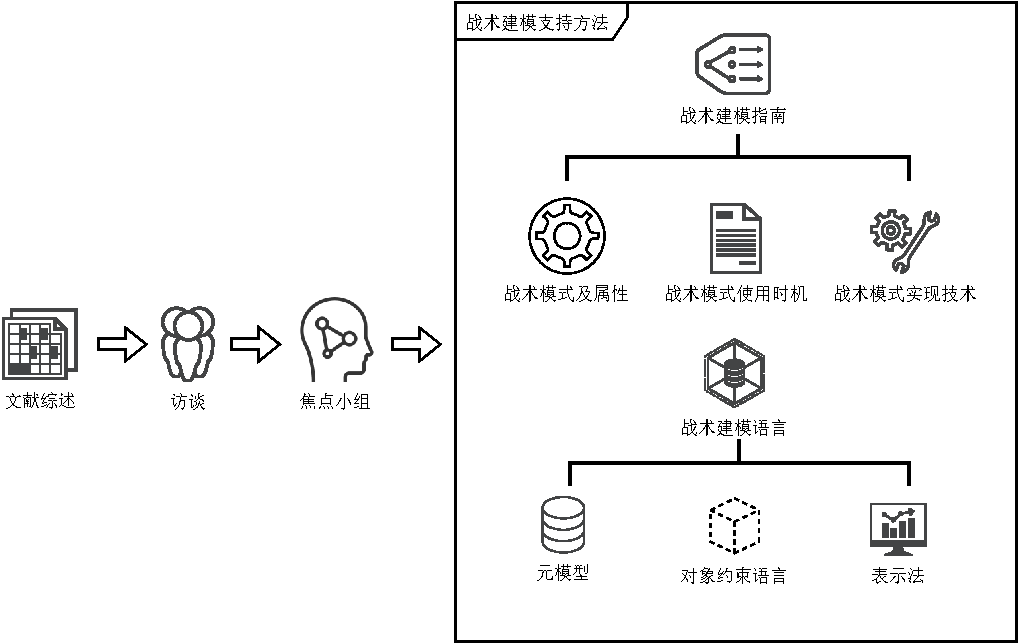
\includegraphics[width=0.8\textwidth]{FIGs/chapter3/researchmethod.pdf} %中括号中的参数是设置图片充满文档的大小,你也可以使用小数来缩小图片的尺寸。
    \caption{战术建模支持方法研究过程图} %caption是用来给图片加上图题的
    \label{researchmethod} %这是添加标签,方便在文章中引用图片。
\end{figure}%figure环境

\section{研究过程}

\subsection{文献综述}

本小节主要介绍文献综述相关工作。
文献综述总结了前人的工作成果,
从领域驱动设计相关著作中进行战术模式的收集与定义。
本工作从战术模式中抽取了重要特征,提高实例化战术建模语言的效率与正确性。
总结了战术建模的使用时机与实现技术,作为战术建模支持方法的一部分。
本工作在调研阶段还参考了相关文献中提出元模型的流程方法,作为元模型构建的理论基础,
对现有领域驱动设计建模元模型的特征进行研究和总结,吸取元模型构建经验。

作者从《领域驱动设计:软件核心复杂性应对之道》\cite{DBLP:books/daglib/0013521}、
《实现领域驱动设计》\cite{vernon2013implementing}两本著作中抽取了八种战术建模模式以及它们的
重要特征,并以此为基础,构建了一个特定于领域驱动设计战术建模的初始元模型。
Evans认为使用领域驱动设计的人员需要经常快速地浏览一些重要的模式,
并掌握这些模式的实施要点和特征,
并与实际业务进行结合使用\cite{evans2014domain}。
领域驱动设计中的概念知识,特别是更为分散的战术模式相关概念知识繁多复杂,需要在使用时经常进行学习和回顾,
确保实践的准确性,
这也是将战术模式属性、使用时机和实现技术纳入建模支持方法的一个重要原因。


在本小节总结的成果中,战术建模模式包括:实体(Entity)、值对象(Value Object)、
领域服务(Domain Service)、领域事件(Domain Event)、聚合(Aggregate)、
资源库(Repository)、模块(Module)、工厂(Factory)。
战术模式重要特征描述了战术模式应该具备的特点、约束条件以及它和不同模式间的关系。
战术模式应用场景描述了每个模式的使用时机和实现时的核心问题。
上述成果将作为访谈问卷的理论基础,经过访谈不断迭代完善,
最终形成关于战术模式的使用指南。

\subsection{访谈}

% 根据文献综述成果,设计问卷问题,
% 对3名工业界内领域驱动设计战术建模的实践者进行访谈并总结访谈结果。
通过分析多次访谈的结果,
对文献综述阶段得到的战术模式进行验证和筛选,
对战术模式重要特征、使用时机和实现技术进行确认和修改,
总结出一套战术建模指南。

访谈活动共进行三次,每次访谈一名对象,访谈持续时间控制在一小时左右。
表\ref{respondents}展示了访谈对象的具体信息,
三名访谈对象分别来自思特沃克、阿里巴巴和华为,
其中有两名架构师和一名开发人员。

{\footnotesize
\begin{longtable}[h]{m{70pt}|m{60pt}|m{255pt}}
    \caption[受访者信息]{受访者信息} \label{respondents} \\
        \hline  
        业务领域&角色&从业经验及年限\\
        \hline
        软件咨询领域&架构师&就职于斯特沃克(ThoughtWorks),
        为国内外医疗、金融、通信、汽车等行业的客户提供软件咨询和交付服务。
        作为技术顾问参与和主导了多次领域驱动设计相关工作,
        是将领域驱动事件风暴引入国内的第一批技术人员。
        拥有10年左右的开发及架构设计经验。\\
        \hline
        通信领域&架构师&就职于华为,
        使用领域驱动设计相关思想与方法多次主导并参与过大型分布式项目的架构设计与微服务拆分。
        拥有10年以上的开发及架构设计经验。\\
        \hline
        电商领域&开发人员&就职于阿里巴巴,
        担任过项目经理,参与过微服务开发,具有战术建模的实践经验,
        对领域驱动设计有过一定了解。
        拥有2年左右的开发及项目管理经验。\\
        \hline

    \end{longtable}
}

访谈首先对访谈对象的个人信息进行了解,包括受访对象的职位、团队规模以及业务领域,
方便对领域驱动设计战术建模实践场景进行评估;
然后对领域驱动设计建模过程进行了解,包括建模使用的工具,建模工作的总体流程,
用来和本文工作做对比,评估本文工作对战术建模领域的作用;
最终聚焦战术建模中的战术模式,对文献综述阶段总结的成果进行评估。
如表\ref{reviewQ}所示,展示了访谈中主要关注的五个方面,
并阐述了具体原因。
具体访谈问卷问题见附录\ref{app:1}。
在访谈中,
受访对象均对本文工作研究内容和最终产出的支持工具持积极态度。

{\footnotesize
\begin{longtable}[h]{m{170pt}|m{215pt}}
    \caption[访谈关注问题]{访谈关注问题} \label{reviewQ} \\
        \hline  
        关注问题&原因\\
        \hline
        何时使用该模式&获取和验证战术模式的使用时机。\\
        \hline
        该模式应该包含哪些重要属性&获取和验证战术模式的属性。\\
        \hline
        实践该模式时有哪些好的实践&获取和验证战术模式的实现技术与细节。\\
        \hline
        实践该模式时有哪些不好的实践&排除不好的实现技术。\\
        \hline
        针对于特定模式的特殊问题&验证对应战术模式是否有必要加入建模支持方法。\\
        \hline
    \end{longtable}
}



\subsection{焦点小组}

本小节介绍研究过程中使用焦点小组形式进行战术建模支持方法构建的相关内容。在所有访谈结束后,
组织焦点小组对文献综述与访谈结果进行分析和评估,目的是不断完善战术建模支持方法内容,
包括迭代和实例化战术建模语言,总结整合战术模式、模式属性、使用时机以及实现技术。

每次焦点小组由包含作者在内的三名研究人员参与,
作者为主持人兼记录员,
负责主持会议和记录会议内容,
其他与会人员均对领域驱动设计相关知识具有一定了解。

如图\ref{focusgroup}所示展示了焦点小组的详细实施过程。
在会议开始前,先将前期文献综述与访谈的成果作为资料展示给参与人员,
并由主持人介绍访谈的初步成果。
会议开始后,使用领域驱动设计战术建模中的重要概念以及会议资料对战术建模支持方法进行设想。
首先,将文献综述和访谈结果中的战术模式与其重要特征进行整合,形成战术模式及其属性列表;
在整合过程中,找出重复和互补的修改建议,使最终战术模式与特征列表更加准确完善,
更好地充当构建战术建模语言时的附加属性;
通过UML profile机制构建元模型,
并设计对象约束语言和建模语言表示方法来实例化战术建模语言;
最后,将战术模式使用时机与实现技术纳入到战术建模指南中;
经过多次焦点小组的讨论和修改后,
战术模式、战术模式的属性、使用时机以及实现技术共同组成了战术建模指南,
汇总战术建模指南和实例化的战术建模语言,形成最终的战术建模支持方法,并对其进行评估。


% 并从访谈结果中抽取战术模式重要特征,找出重复和互相补充的修改建议,形成汇总之后的修改结果,
% 修改后的结果包括战术模式的特征与属性、战术模式之间的关系与约束以及战术建模的实践经验;
% 对总结的结果进行评价,
% 经过多次焦点小组后,使用元模型构建方法(UML profile机制)将修改后的结果添加到元模型中,
% 使用对象约束语言等方式完善建模语言并将新的战术建模实践经验加入到框架中,
% 最终产出一套完整的战术建模框架,整个过程如图\ref{focusgroup}所示。

\begin{figure}[!htbp] %figure环境,h默认参数是可以浮动,不是固定在当前位置。如果要不浮动,你就可以使用大写float宏包的H参数,固定图片在当前位置,禁止浮动。
    \centering %使图片居中显示
    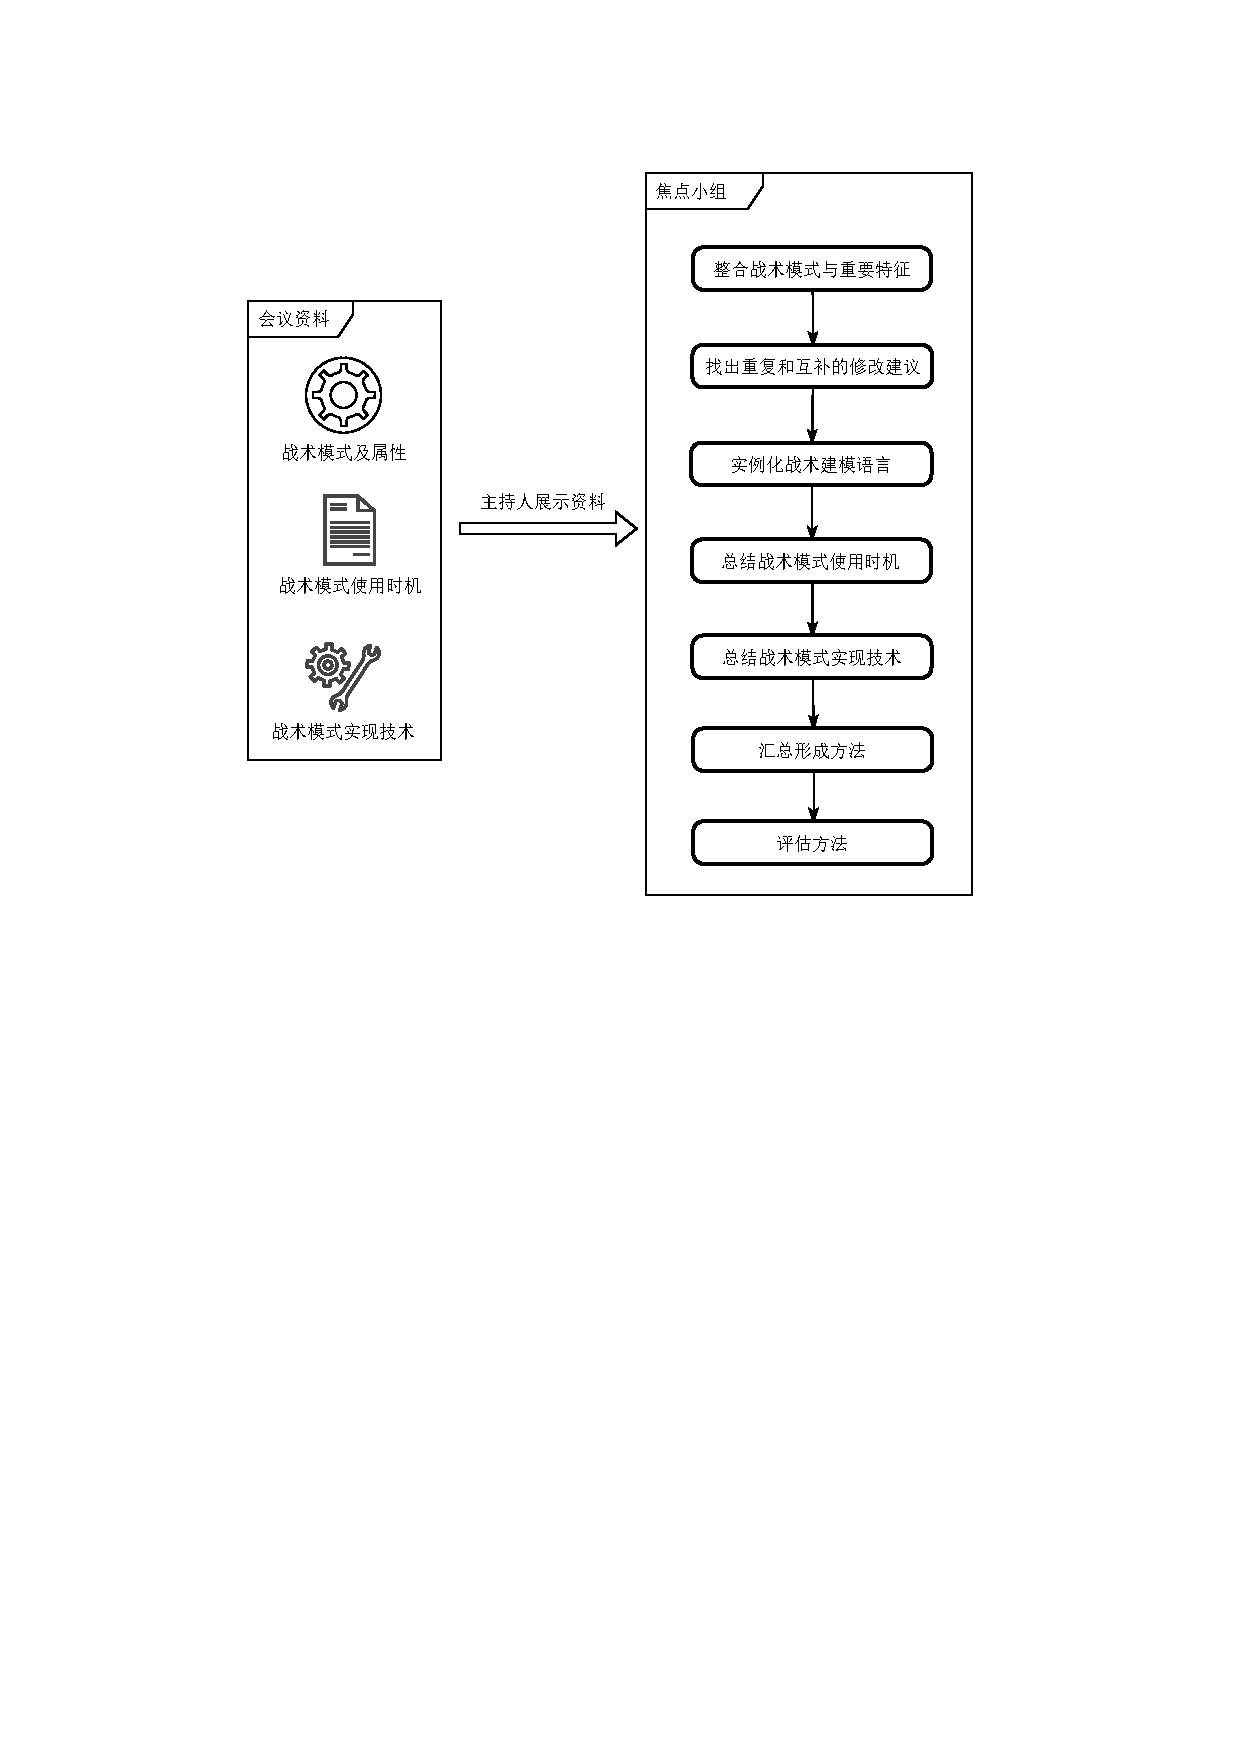
\includegraphics[width=0.8\textwidth]{FIGs/chapter3/focusgroup.pdf} %中括号中的参数是设置图片充满文档的大小,你也可以使用小数来缩小图片的尺寸。
    \caption{焦点小组实施过程} %caption是用来给图片加上图题的
    \label{focusgroup} %这是添加标签,方便在文章中引用图片。
\end{figure}%figure环境

\section{战术建模指南}

\subsection{战术建模模式及属性}

经过文献综述调研工作和对多次访谈的结果进行分析,
总结出了八种战术模式及属性。
作者发现有些原本属于战略建模设计的概念在战术建模时也会纳入考虑范围,
例如,防腐层(Anti-Corruption Layer,ACL)往往会在战术建模时经常使用,
用来隔离和代理对其他限界上下文的访问行为。
此外,战术模式在实现时与理论概念稍有不同,
在真正进行战术建模时,模块(Module)这一模式更多的是代码层面的组织和结构要求,
而非建模时设计阶段需要考虑的因素;工厂(Factory)则与设计模式中的工厂区别不大,
作为建模中的模式意义不大,完全可以作为实现的一种方式,故对这两种模式进行排除,
表\ref{table:patterns}展示了战术建模中的主要模式和它们的重要属性,
其中战术模式的属性以英文单词“Characteristic”的前两位大写字母“CH”结合序号进行编号,
并对每个战术模式的属性进行描述。


{\footnotesize
\begin{longtable}[h]{m{70pt}|m{100pt}|m{210pt}}% 通过添加 | 来表示是否需要绘制竖线
    \caption[战术建模模式及属性]{战术建模模式及属性} \label{table:patterns} \\
        \hline  % 在表格最上方绘制横线
        模式&属性&描述\\
        \hline  %在第一行和第二行之间绘制横线
        \multirow{2}*{\shortstack{实体}}&CH1:唯一标识&实体是唯一的,需要借助唯一标识进行区分和跟踪变化。\\
        \cline{2-3}  %为第二列到第三列添加横线
        &CH2:可变性&实体在其生命周期中是可变的,除唯一标识外都可以进行修改,不管如何变化都可以通过唯一标识进行跟踪。\\
    
        \hline  
        \multirow{5}*{\shortstack{值对象}}&CH3:不变性&值对象创建后不可改变。只有初始化时才能修改对象的属性状态。\\
        \cline{2-3}  
        &CH4:可替换性&值对象无法继续正确表达状态时,度量和描述改变,可以用另一个值对象直接替换。\\
        \cline{2-3}  
        &CH5:值对象相等性&系统中存在很多相等的值对象实例,但它们不是同一个值对象,相等性通过比较两个对象的类型和属性来决定。\\
        \cline{2-3}  
        &CH6:无副作用行为&值对象的所有方法必须只产生输出,而无法改变对象状态,防止破坏不变性。\\
        \cline{2-3}  
        &CH7:概念整体&值对象可以处理一组关联的属性,将它们视为整体。\\
        
        \hline
        \multirow{3}*{\shortstack{领域服务}}&CH8:无状态&服务本身不保存任何数据。\\
        \cline{2-3}  
        &CH9:输入&领域服务的输入参数。\\
        \cline{2-3}  
        &CH10:输出&领域服务的输出结果。\\
    
        \hline
        \multirow{3}*{\shortstack{领域事件}}&CH11:触发时间&领域事件是过去发生的,需要一个时间戳来记录发生事件。\\
        \cline{2-3}  
        &CH12:事件发送方&产生该领域事件的对象和其他参与操作的对象。\\
        \cline{2-3}
        &CH13:不变性&领域事件携带的属性反映过去的信息,不应该再改变。\\
        \cline{2-3}
        &CH14:唯一标识&将领域事件建模成聚合,发布到外部限界上下文时,都需要唯一标识来进行区分、跟踪或去重。\\
    
        \hline
        \multirow{2}*{\shortstack{聚合}}&CH15:根实体&根实体是访问其他聚合的媒介,相当于聚合的“唯一标识”,尽量包含最少的属性。\\
        \cline{2-3}  
        &CH16:一致性边界&聚合是一个原子性的整体,聚合边界内部的所有对象都应该保持一致性,聚合的所有操作都是事务的。\\
        \cline{2-3}  
    
        \hline
        \multirow{2}*{\shortstack{资源库}}&CH17:为聚合根提供&理想条件下只为聚合根提供资源库,但有时也可为实体提供。\\
        \cline{2-3}  
        &CH18:额外行为&不包含业务逻辑的额外行为,如计算总数,特殊化查询方法等。\\
        \hline
\end{longtable} 
}

\subsection{战术建模模式使用时机与实现技术}

结合前期文献综述和访谈结果,
总结出了战术模式在实现时的技术经验与指导准则,
并整合到战术建模支持方法中,
从各种模式的使用时机和实现技术两个方面进行阐述,
为战术建模使用人员界定模式使用场景和时间提供参考,
为战术建模落地实现提供快速解决方案。

如表\ref{patternsTime}所示为战术模式使用时机表,
其中各个战术模式的使用时机以单词“Time”的首字母“T”结合序号进行编号,并进行描述。

{\footnotesize
\begin{longtable}[h]{m{70pt}|m{315pt}}
    \caption[战术模式使用时机]{战术模式使用时机} \label{patternsTime} \\
        \hline  
        模式&使用时机\\
        \hline
        实体&T1:需要将对象和其他对象进行区分时
        \newline T2:需要跟踪对象变化时
        \newline T3:涉及到对象持久化操作时\\
        \hline
        值对象&T4:该对象具有明显的可替换性
        \newline T5:该对象具有不可变的特性\\
        \hline
        领域服务&T6:一个显著的业务操作过程不属于实体或值对象职责时
        \newline T7:一个含有业务含义的领域对象转换过程不属于实体或值对象职责时\\
        \hline
        领域事件&T8:需要捕获发生在领域中的一些重要事件时
        \newline T9:需要维护跨越不同聚合或限界上下文间事件的一致性时\\
        \hline
        模块&T10:将内聚类放在相同模块进行管理
        \newline T11:将没有联系的类放在不同模块进行解耦合\\
        \hline
        聚合&T12:需要将实体和值对象聚类到一致性边界内时
        \newline T13:需要保证密切关联的一组对象内部的不变条件时\\
        \hline
        资源库&T14:聚合实例可以放在资源库中,保证存取同一个聚合
        \newline T15:存储需要进行全局访问的对象
        \newline T16:严格来说只为聚合提供,但有时也可以为实体提供\\
        \hline
\end{longtable}
}

战术模式实现技术对各个模式进行实现时采用的技术进行了描述和编号,
其中实现技术及方案以单词“Practice”的首字母“P”结合序号进行编号,
并给出了实现时推荐的技术方案与具体细节。具体内容如下:


\textbf{实体实现技术及方案}

P1:生成唯一标识
\begin{itemize}[leftmargin = 40pt]
    \item 用户提供唯一的一个或多个初始值作为输入的唯一标识。该方式简单直接,但有时保证用户提供的标识唯一很困难。
    \item 应用程序生成唯一标识。该方式能生成有明确意义的可读标识,且程序生成的方式保证了全局唯一性。
    \item 持久化机制生成唯一标识。该方式将生成标识的职责委派给持久化机制(如数据库),结果保证唯一,但耗时较长,成功率依赖持久化机制稳定性。
\end{itemize}

P2:唯一标识生成时间
\begin{itemize}[leftmargin = 40pt]
    \item 创建对象时生成(及早生成)。如果需要发布领域事件,就要尽早地在发布前就生成,以便标识领域事件;在未持久化之前需要进行区分时,也要尽早生成唯一标识。
    \item 对象持久化时生成唯一标识。除上述情况外,都可以在对象持久化时再生成唯一标识。
\end{itemize}

P3:保持唯一标识稳定性的方法
\begin{itemize}[leftmargin = 40pt]
    \item 将设置唯一标识的方法隐藏,让外部无法访问;设置唯一标识前询问是否存在,如存在则禁止更新。
\end{itemize}

\textbf{值对象实现技术及方案}

P4:保证值对象不变性
\begin{itemize}[leftmargin = 40pt]
    \item 只允许初始化时设置值对象属性。
\end{itemize}

P5:存储值对象集合的方法
\begin{itemize}[leftmargin = 40pt]
    \item 多个值对象序列化到单个列中。该方式将集合序列化为单列文本,序列化后的对象无法支持查询,且需要持久化机制支持较长单列长度。
    \item 将值对象转化为数据库实体。该方式将多个值对象共同关联的实体的唯一标识作为主键,相当于将值对象在持久化层次变成了“实体”。
\end{itemize}

\textbf{领域服务实现技术及方案}

P6:实现领域服务
\begin{itemize}[leftmargin = 40pt]
    \item 抽象一个接口。该方式适合有多种实现类的领域服务。
    \item 直接定义实现类。该方式适合逻辑简单、无需定义接口的领域服务。
    \item 只关注业务逻辑。领域服务只关注业务逻辑和流程,不依赖特定实现技术或持久化机制。
\end{itemize}


\textbf{领域事件实现技术及方案}

P7:实现领域事件

\begin{itemize}[leftmargin = 40pt]
    \item 聚合创建事件并发布事件。
    \item 事件订阅方直接转发或先存储再转发到远程订阅方,如果消息中间件没有和模型共享数据存储,要使用两阶段提交(Two-Phase Commit,2PC),确保最终一致性。
    \item 尽量避免过度暴露领域模型给消息设施。
    \item 保证订阅方在事件发布前完成订阅,确保能够接收事件。
    \item 资源库禁止删除已存储事件,因为事件表示已发生的既定事实。
    \item 如图\ref{DomainEventPractice}所示描述了实现领域事件过程的流程图。
\end{itemize}

\begin{figure}[h] %figure环境,h默认参数是可以浮动,不是固定在当前位置。如果要不浮动,你就可以使用大写float宏包的H参数,固定图片在当前位置,禁止浮动。
    \centering %使图片居中显示
    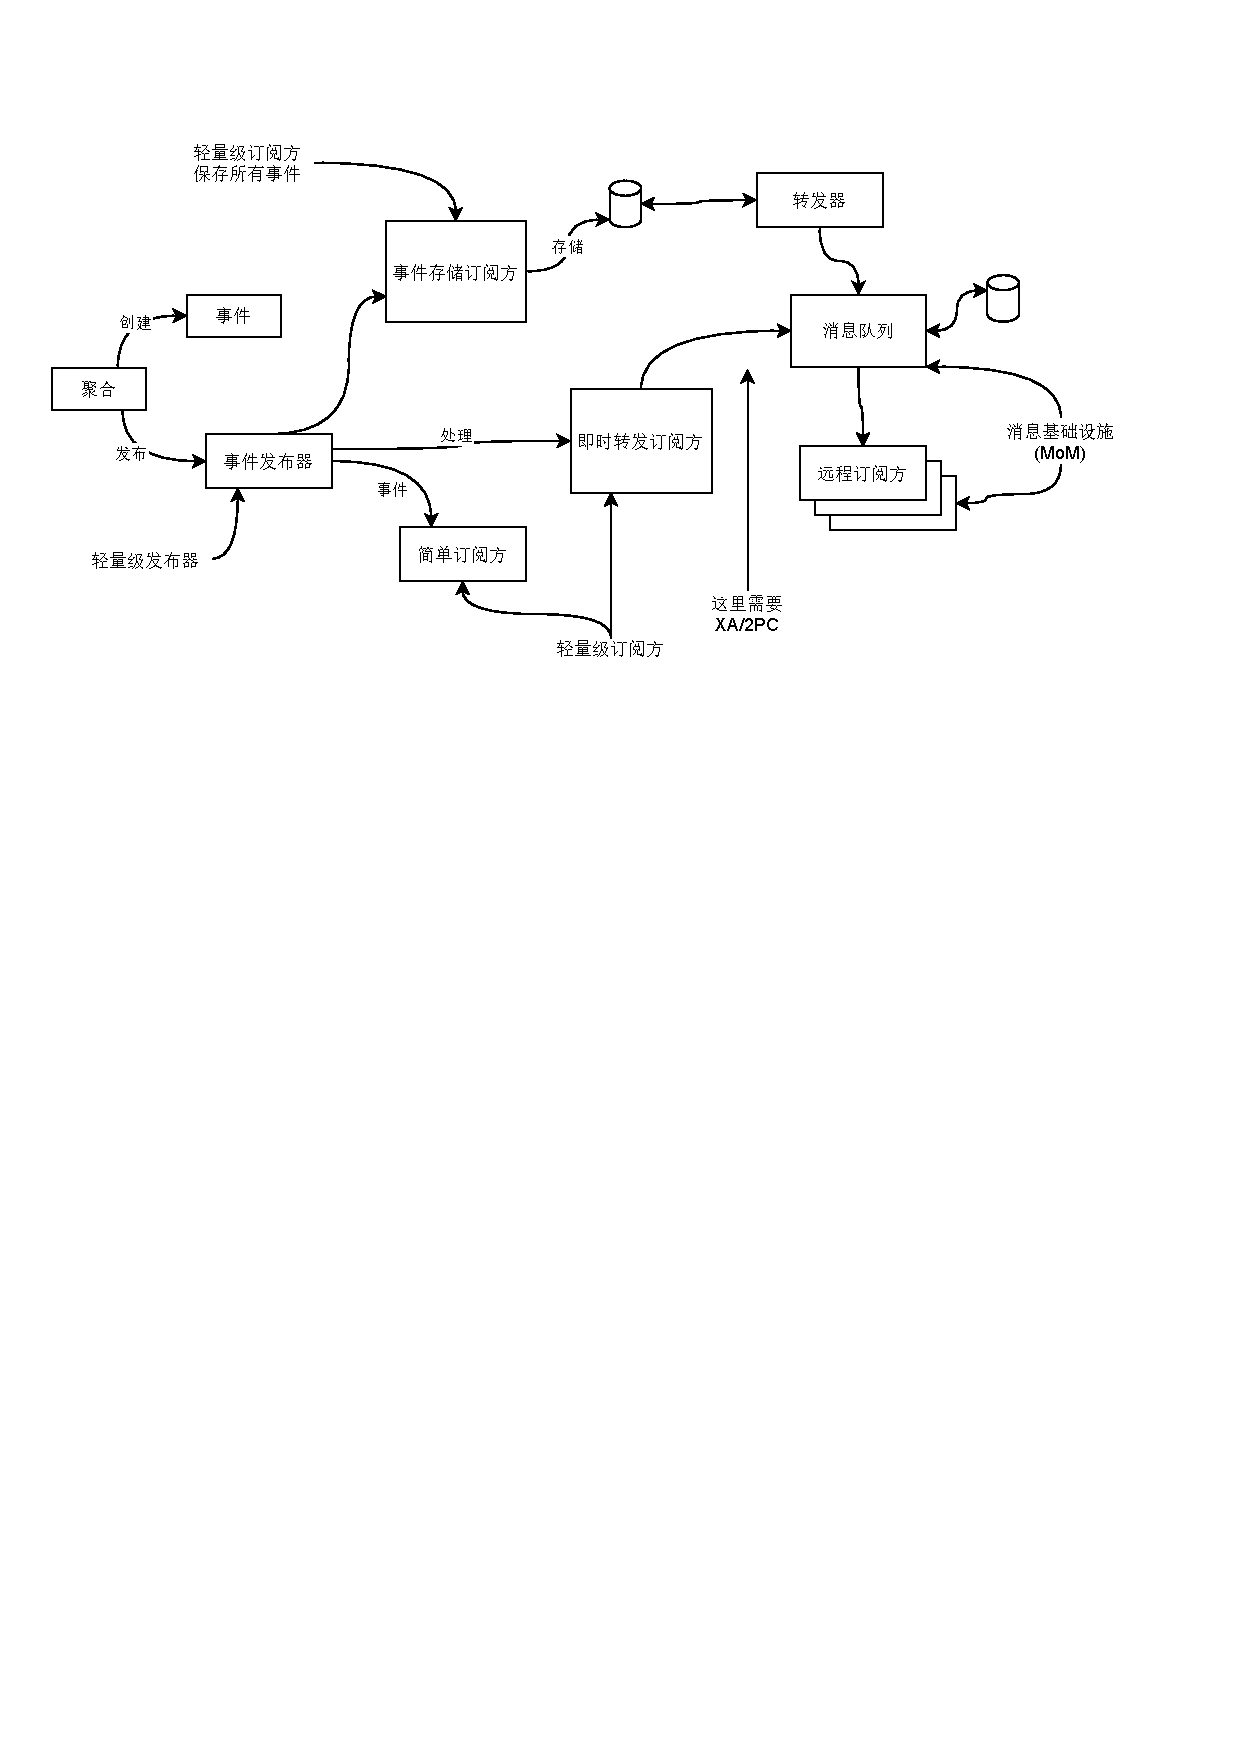
\includegraphics[width=0.8\textwidth]{FIGs/chapter3/DomainEventPractice.pdf} %中括号中的参数是设置图片充满文档的大小,你也可以使用小数来缩小图片的尺寸。
    \caption{领域事件实现流程图\protect\footnotemark[1]} %caption是用来给图片加上图题的
    \label{DomainEventPractice} %这是添加标签,方便在文章中引用图片。
\end{figure}%figure环境
\footnotetext[1]{图片来源于《实现领域驱动设计》}

P8:保持领域事件不变性
\begin{itemize}[leftmargin = 40pt]
    \item 只允许领域事件全状态初始化,避免初始化后又进行修改。
    \item 避免领域模型暴露到消息设施,防止第三方进行修改。
\end{itemize}

P9:转发领域事件
\begin{itemize}[leftmargin = 40pt]
    \item 通过RESTful接口发布。该方式适合多个客户同时通过相同URL请求来获取事件通知,不关注事件通知的顺序。
    \item 通过消息中间件方式发布。该方式依赖消息中间件省去细节处理,只需确保推送消息成功。
\end{itemize}

\textbf{模块实现技术及方案}

P10:组织模块
\begin{itemize}[leftmargin = 40pt]
    \item 不要只根据通用组件所属战术模式类型来组织模块,即不要简单地将所有聚合放在同一个模块,所有领域服务放在同一个模块,要考虑业务逻辑与行为。
    \item 设计松散耦合的模块,有利于维护和重构模块。
    \item 同层模块出现耦合时,杜绝循环依赖。
    \item 模块与建模对象一同变化,模型中对象改变时,模块也应进行改变。
\end{itemize}

\textbf{聚合实现技术及方案}

P11:保证一致性边界
\begin{itemize}[leftmargin = 40pt]
    \item 用事务来保证一致性边界。事务一致性要求立即性和原子性,提交单个事务时,聚合边界内的所有内容都必须保持一致。
\end{itemize}

P12:设计聚合的原则
\begin{itemize}[leftmargin = 40pt]
    \item 设计小聚合。使用根实体代表聚合,只包含最小数量的属性(需要在领域内保持一致性的属性)。
    \item 聚合内部建模成值对象。值对象可以配合根实体一同序列化存储,不会带来不必要的操作。
\end{itemize}

\textbf{资源库实现技术及方案}

P13:实现资源库
\begin{itemize}[leftmargin = 40pt]
    \item 为存储的聚合或实体提供访问的全局接口,确保存取的便捷性。
    \item 提供添加和删除方法。
    \item 提供顺序自增的唯一标识。
\end{itemize}

\subsection{战术建模指南构建结果}

本小节将介绍基于文献综述和访谈结果,
通过焦点小组讨论构建的战术建模指南。
指南中各模式包含的内容如表\ref{modelingframework}所示。
战术建模指南包含各个模式的名称、特征属性、使用时机和实现技术方案,
为方便表示,以上内容均以编号代表。


{\footnotesize
\begin{longtable}[h]{m{70pt}|m{125pt}|m{100pt}|m{75pt}}
    \caption[战术模式包含内容]{战术模式包含内容} \label{modelingframework} \\
        \hline  
        模式&属性&使用时机&实现技术\\
        \hline
        实体&CH1 CH2&T1 T2 T3&P1 P2 P3\\
        \hline
        值对象&CH3 CH4 CH5 CH6 CH7& T4 T5 &P4 P5\\
        \hline
        领域服务&CH8 CH9 CH10& T6 T7 &P6\\
        \hline
        领域事件&CH11 CH12 CH13 CH14&T8 T9&P7 P8 P9\\
        \hline
        模块&无&T10 T11&P10\\
        \hline
        聚合&CH15 CH16& T12 T13&P11 P12\\
        \hline
        资源库&CH17 CH18& T14 T15 T16& P13\\
        \hline

\end{longtable}
}

形成的具体战术建模指南如图\ref{theoryFramework}所示。
建模指南按模式划分,
每个模式包含了属性、实现技术及使用时机,
每个属性使用虚线关联其对应的实现技术。
为方便表示,以上内容均以编号代表。
该建模指南可以作为战术建模全流程的标准化参考。


\begin{figure}[!htbp] %figure环境,h默认参数是可以浮动,不是固定在当前位置。如果要不浮动,你就可以使用大写float宏包的H参数,固定图片在当前位置,禁止浮动。
    \centering %使图片居中显示
    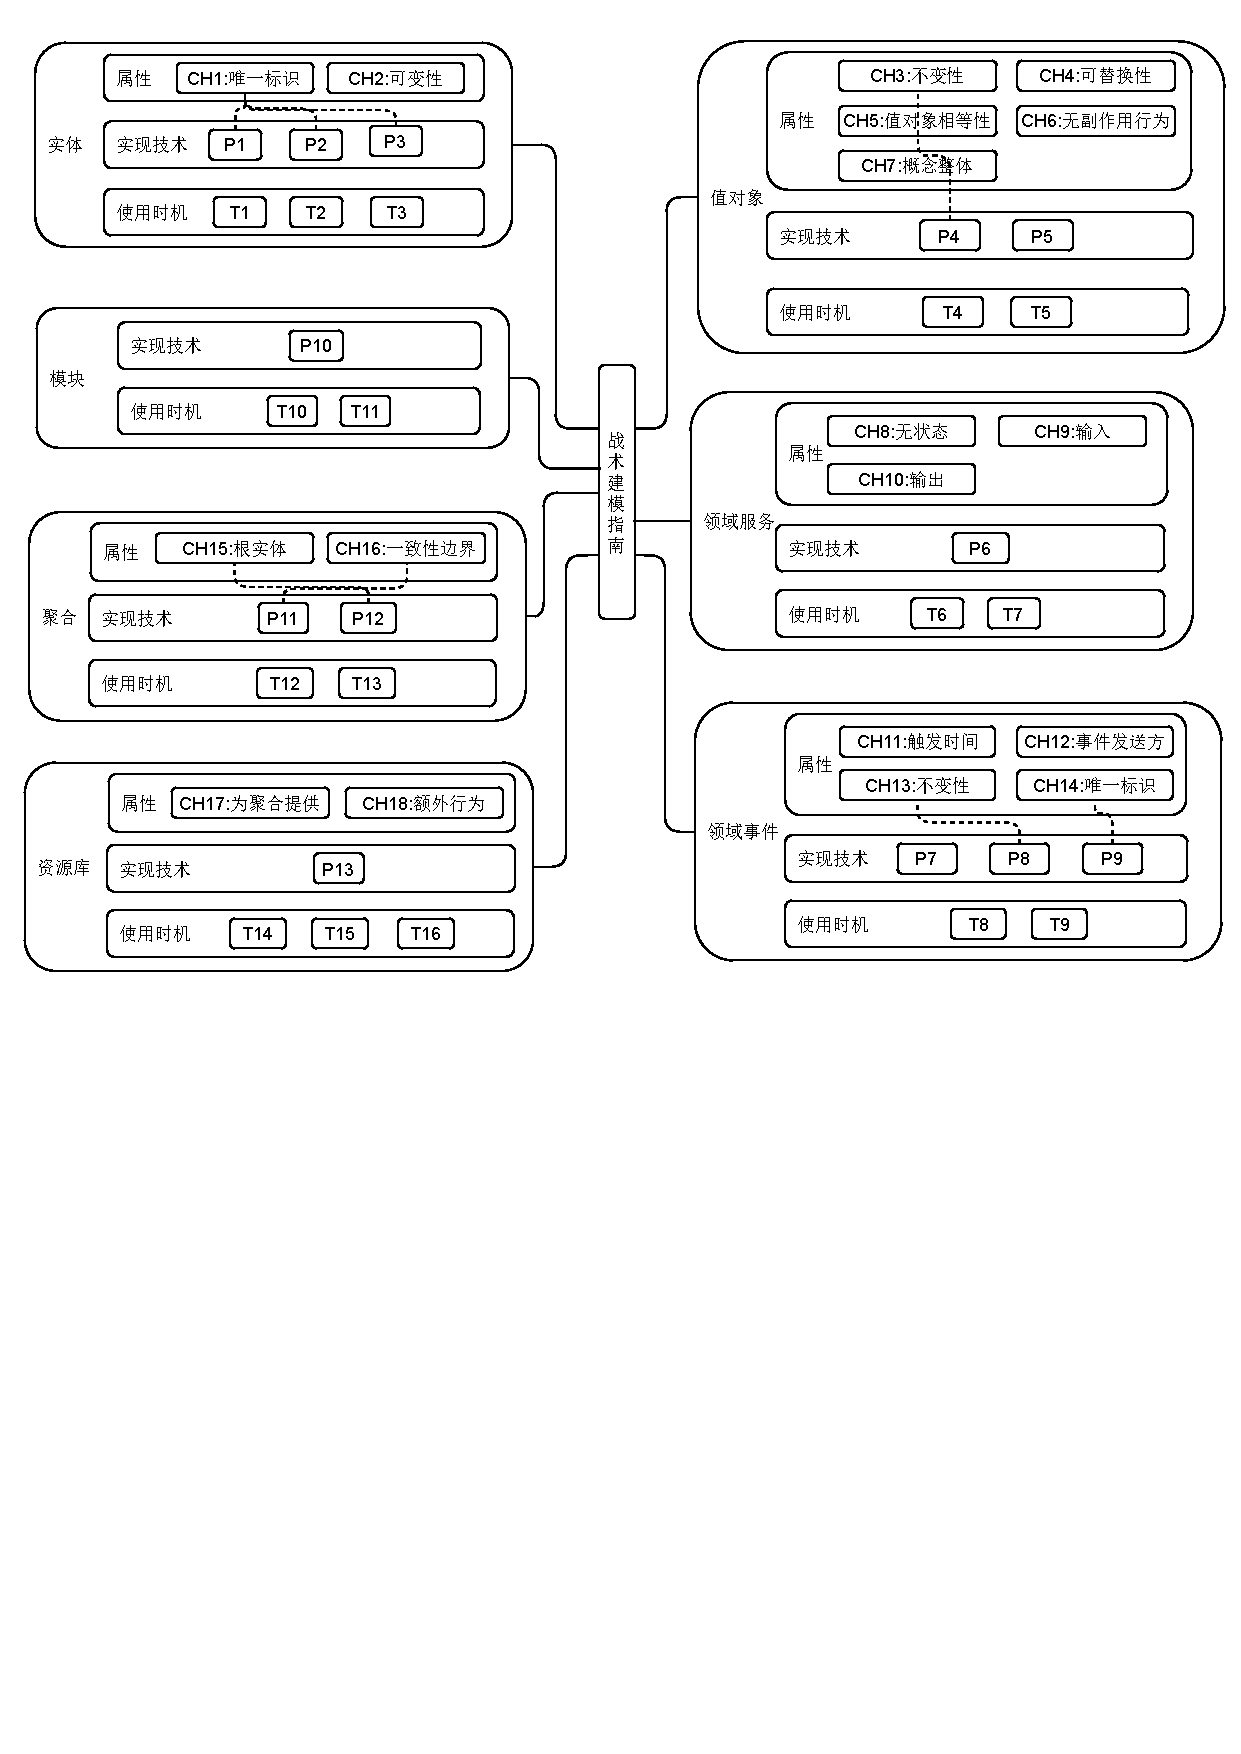
\includegraphics[width=0.8\textwidth]{FIGs/chapter3/theoryFramework.pdf} %中括号中的参数是设置图片充满文档的大小,你也可以使用小数来缩小图片的尺寸。
    \caption{战术建模指南} %caption是用来给图片加上图题的
    \label{theoryFramework} %这是添加标签,方便在文章中引用图片。
\end{figure}%figure环境

\section{战术建模语言}

% 战术建模框架本身应该是基于review和访谈结果总结得到的一个战术建模方法,想想看它应该包含哪些内容

本节将介绍基于焦点小组讨论实例化的战术建模语言。
作者实例化建模语言的过程参考了\cite{giachetti2009integration,giachetti2009using}文献中的流程方法,
提出的元模型参考了\cite{hippchen2019systematic,le2018domain,rademacher2017towards}文献中的现有元模型。
首先使用UML profile机制来进行战术建模元模型的构建,
包括战术建模初始元素集的构建,
初始元素集展示了建模语言中需要使用的重要概念,
并与元类类型对应;
还构建了战术建模元类,
UML中的元类是一种成熟的元模型实现方式,
由于UML类图与软件设计实现关系密切,并且易于阅读理解,
所以以其为重点进行UML profile的构建;
然后使用对象约束语言(OCL)对约束条件进行实现,
对象约束语言(OCL)是一种施加在指定模型元素上的约束语言,
为元模型附加了更多约束条件使其更加完善。


\subsection{战术建模语言元素集}

根据表\ref{table:patterns}定义战术建模UML profile元模型(Metamodel)需要的元素集。
本文定义的元素集如表\ref{ProfileElementSet}所示,
表中展示了元素集中元素的名称,代表的元类类型以及描述。

{\footnotesize
\begin{longtable}[h]{m{80pt}|m{90pt}|m{205pt}}
\caption[战术建模profile元素集]{战术建模profile元素集} \label{ProfileElementSet} \\
    \hline  
    元素名&元类类型&描述\\
    \hline
    Entity&Class&实体是一个由标识符定义的对象,通过标识符与其他对象区别开来确保其个性特征。\\
    \hline
    ValueObject&Class&值对象用来度量和描述事物,具有不可变性。\\
    \hline
    DomainService&Class&领域服务是一个独立接口或对象,负责承担不属于实体或值对象职责的操作或转换过程。\\
    \hline
    DomainEvent&Class&领域事件记录了领域中发生的事情,无法改变,还可以维护发布到外部上下文的业务一致性。\\
    \hline
    AggregateRoot&Class&聚合是一个将实体和值对象聚类到一致性边界内的容器,每个聚合内部有一个实体作为聚合根,
    聚合通过聚合根与外部进行交互。\\
    \hline
    Repository&Class&资源库是一个用来存取领域对象的安全存储区域,还可以提供对象的存取、删除和查询操作。\\
    \hline
    DefineIdentity&Property or Operation&唯一标识,用来区分其他对象和跟踪对象。\\
    \hline
    Module&Package&模块是用来存放内聚类的容器,主要用在技术层面的代码组织、构建目录与打包。\\
    \hline
    Input&Class and Property&领域服务对象或领域事件对象方法的输入。\\
    \hline
    Output&Class and Property&领域服务对象方法的输出。\\   
    \hline
    OccurTime&Property&领域事件触发时间。\\
    \hline
    EventStep&Property or Operation&事件步骤,用来描述领域事件。\\
    \hline
    ACL&Class&防腐层,用来和其他上下文交互和隔离。\\
    \hline
\end{longtable} 
}

如表\ref{ProfileElementSet}所示,在重要战术模式表\ref{table:patterns}的基础上,
进行了优化与修改。
直接用聚合根(AggregateRoot)和与聚合根直接或间接相连的所有对象表示聚合(Aggregate),
为领域服务(Domain Service)引入必要属性输入(Input)和输出(Output),
为领域事件(Domain Event)引入必要属性输入(Input)来代表发送方,
还引入了触发时间(OccurTime)和领域事件步骤(EventStep)属性。
引入严格意义上不是战术模式但可能会用到的概念元素防腐层(Anti-Corruption Layer,ACL)。

\subsection{战术建模元类}

一个UML profile包含构造型(Stereotypes)形式的UML元类的扩展,
还包含元类中类(Class)、属性(Property)和操作(Operation)的映射关系
\cite{files2013omg},
使用定义好的配置文件构造型,可以对元类进行扩展,丰富其语义。
如图\ref{metaclass}描述了扩展元类的战术建模UML profile,包含所有的构造型,
以及各构造型之间的包含关系,采用标记值(Tagged Values)进行表示。
其中,箭头表示构造型扩展自元类。

\begin{figure}[!htb] %figure环境,h默认参数是可以浮动,不是固定在当前位置。如果要不浮动,你就可以使用大写float宏包的H参数,固定图片在当前位置,禁止浮动。
    \centering %使图片居中显示
    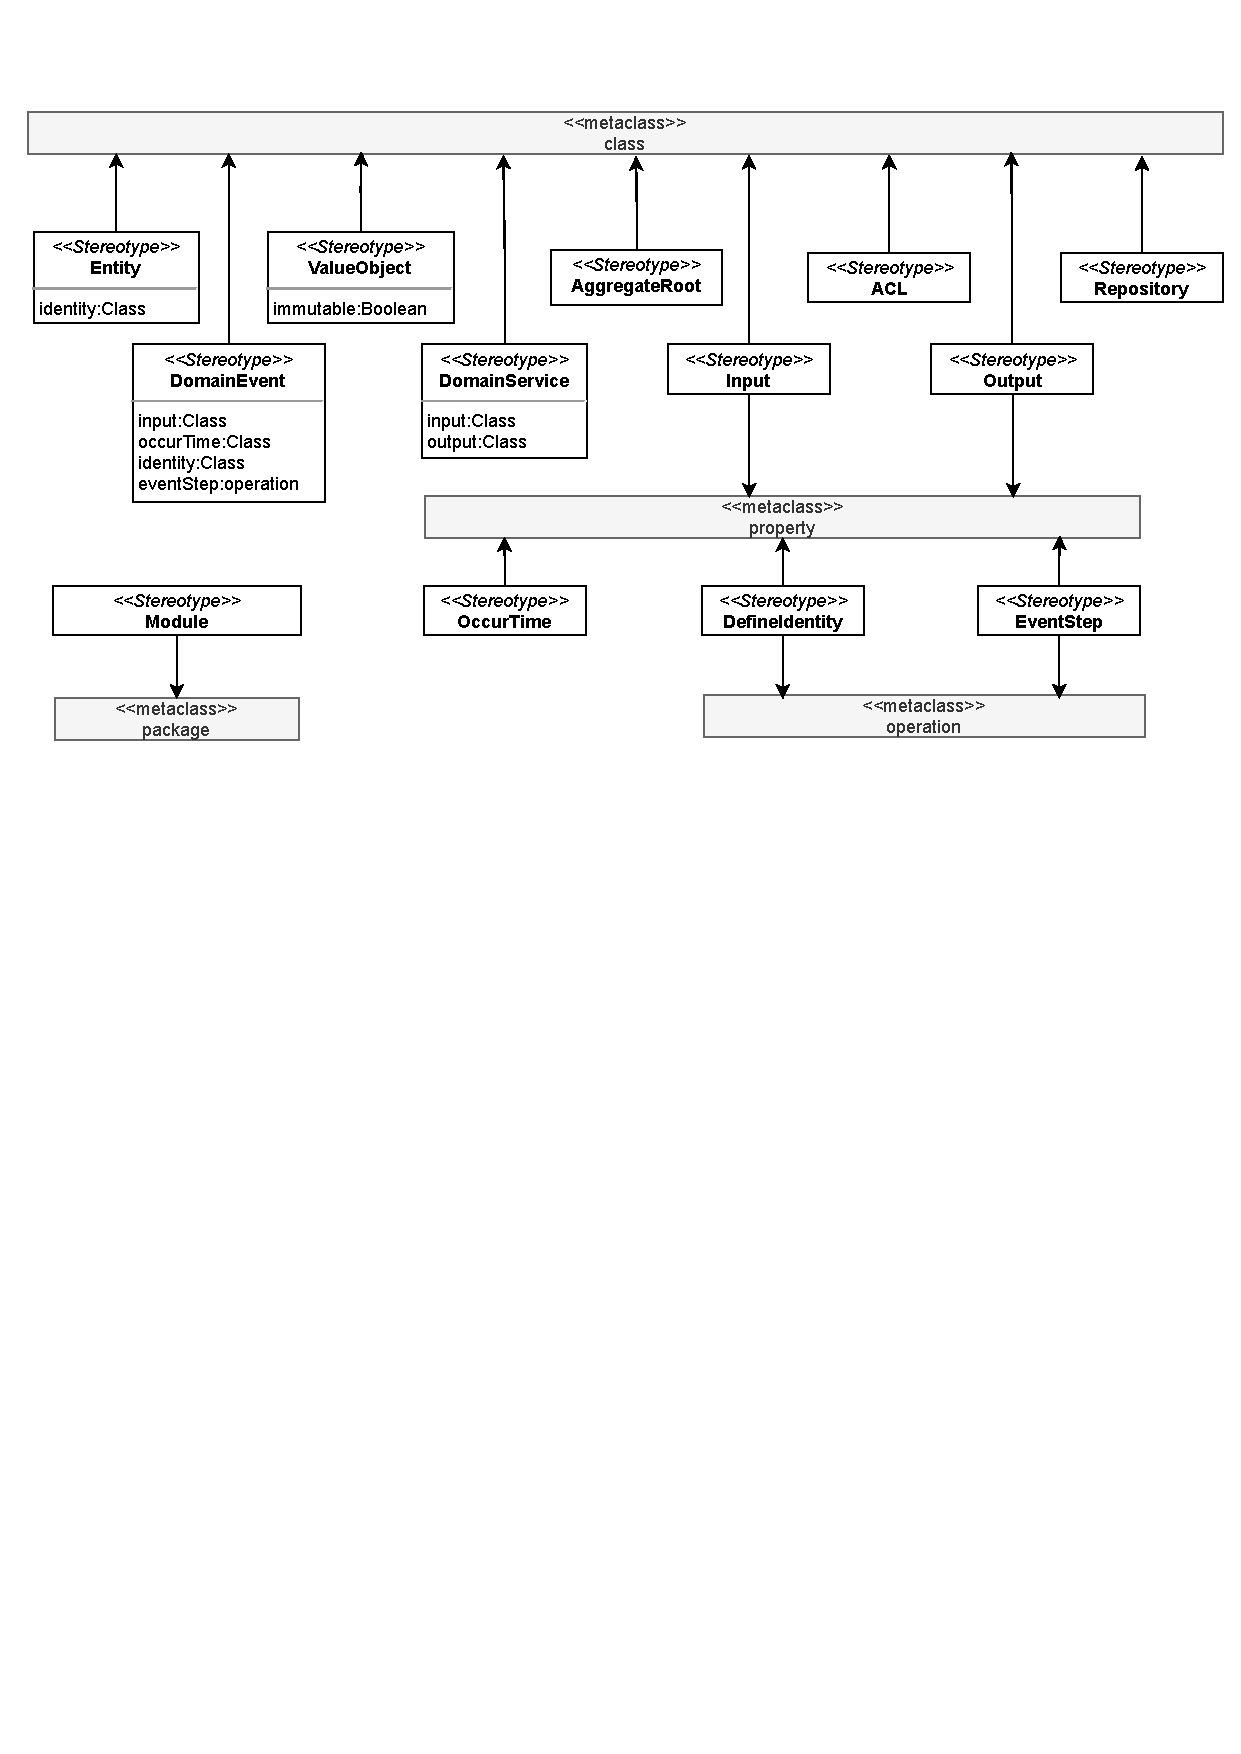
\includegraphics[width=0.8\textwidth]{FIGs/chapter3/metaclass.pdf} %中括号中的参数是设置图片充满文档的大小,你也可以使用小数来缩小图片的尺寸。
    \caption{战术建模扩展元类profile} %caption是用来给图片加上图题的
    \label{metaclass} %这是添加标签,方便在文章中引用图片。
\end{figure}%figure环境

\subsection{战术建模语言约束}

为元类添加约束可以防止不规范或错误使用元类,
为确保上述扩展元类正常使用以及建模过程的准确性,
每个元类都被添加了相应约束,具体约束如表\ref{stereotypeconstraint}所示,
使用英文单词“Constraint”的大写首字母“C”结合序号对约束进行编号,
并通过对象约束语言对约束进行标准化的实现。

% 结合profile的拓展机制形成的元模型
% 特征,约束和规则,表格形式

{\footnotesize
\begin{longtable}[h]{m{90pt}|m{295pt}}
    \caption[构造型约束规则]{构造型约束规则} \label{stereotypeconstraint} \\
        \hline  
        构造型&约束\\
        \hline
        Entity&C1:实体必须拥有一个方法或属性定义唯一标识。\\
        \hline
        DomainService&C2:领域服务类不能具有其他构造型。
        \newline C3:领域服务必须拥有输入值。
        \newline C4:领域服务必须拥有输出值。\\
        \hline
        DomainEvent&C5:领域事件类不能具有其他构造型。
        \newline C6:领域事件必须记录被触发时间。
        \newline C7:领域事件必须拥有事件发送方作为输入。
        \newline C8:领域事件必须拥有唯一标识来跟其他对象进行区分。\\
        \hline
        AggregateRoot&C9:只有实体能充当聚合根并与其他聚合根连接。
        \newline C10:一个聚合根只能由一个实体代表。\\
        \hline
        Repository&C11:资源库类不能具有其他构造型。
        \newline C12:只为实体或聚合根提供资源库。
        \newline C13:资源库只定义方法,且至少定义一个方法。
        \\
        \hline
        ValueObject&C14:值对象不可变。\\
        \hline
        DefinesIdentity&C15:唯一标识可以以属性或方法返回值的形式存在于对象中。
        \newline C16:唯一标识必须在实体或领域事件中使用。\\
        \hline
        Input&C17:输入以属性形式存在于对象中,且必须指定输入代表的对象。\\
        \hline
        Output&C18:输出以属性形式存在于对象中,且必须指定输出代表的对象。\\   
        \hline
        OccurTime&C19:触发时间必须作为属性在领域事件中使用。\\
        \hline
    \end{longtable} 
}
% 使用OCL时运用到了以JavaScript\footnote{JavaScript主页:https://www.javascript.com/}
% 为基础的开源工具包OCL.js\footnote{OCL.js开源项目仓库:https://github.com/SteKoe/ocl.js}。
% 使用该工具后,可以直接将OCL语句集成到前端项目代码中,达到校验约束、方便查看的效果。
对象约束语言(OCL)可以施加在指定元类上,
为元类附加更多约束条件,
使其在使用过程中更加标准规范,避免错误地使用元类。
由于本文篇幅有限,仅选择领域事件的约束实现进行展示,
如图\ref{DomainEventOCL}所示,展示了用OCL实现的领域事件约束。\\

\begin{figure}[!htbp] %figure环境,h默认参数是可以浮动,不是固定在当前位置。如果要不浮动,你就可以使用大写float宏包的H参数,固定图片在当前位置,禁止浮动。
    \centering %使图片居中显示
    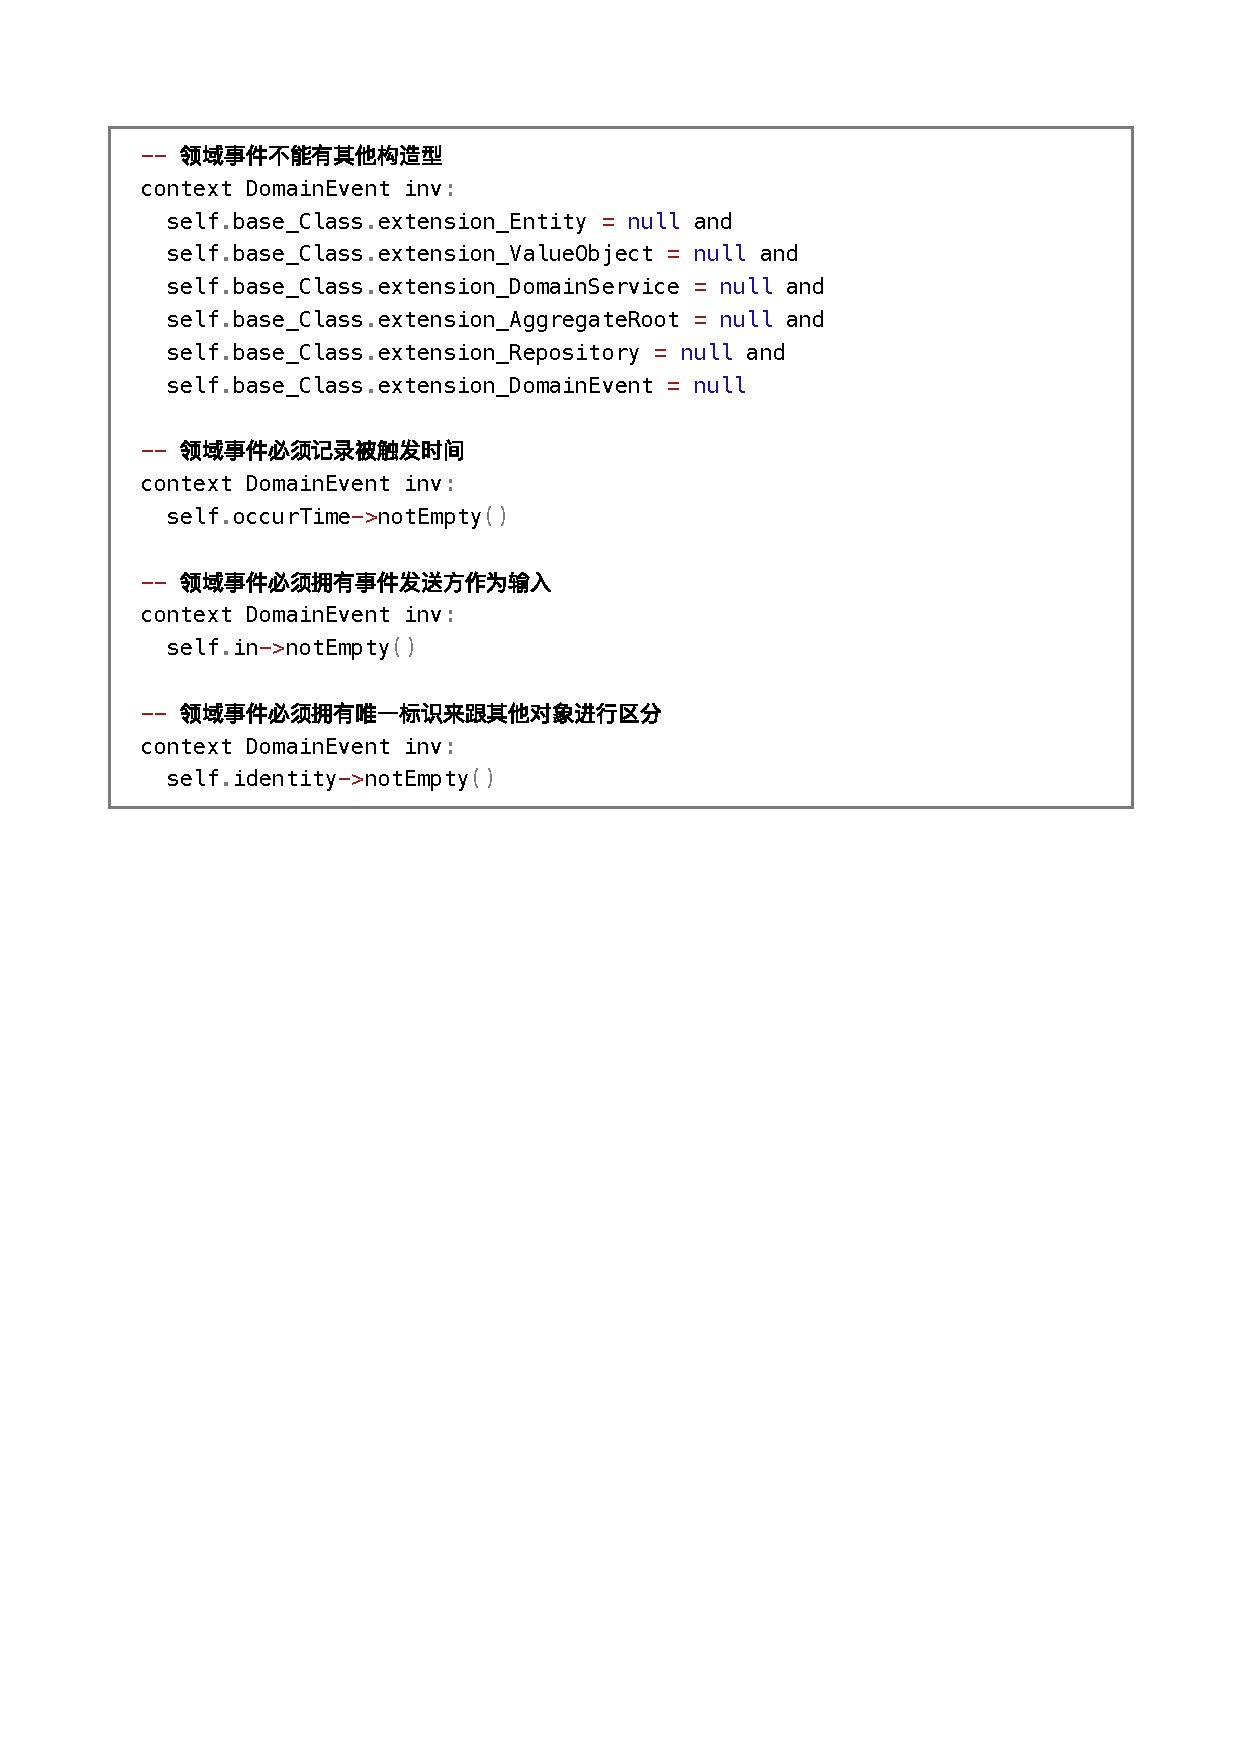
\includegraphics[width=0.8\textwidth]{FIGs/chapter3/DomainEventOCL.pdf} %中括号中的参数是设置图片充满文档的大小,你也可以使用小数来缩小图片的尺寸。
    \caption{DomainEvent约束实现} %caption是用来给图片加上图题的
    \label{DomainEventOCL} %这是添加标签,方便在文章中引用图片。
\end{figure}%figure环境

% \subsection{战术建模最佳实践经验}


% \subsection{支持工具}

% 支持框架的工具使用流程如下图\ref{toolprocess}所示。
% 开发者使用支持工具开始建模,首先可以选择学习或回顾DDD基本概念知识,
% 为后续建模做理论准备,也可以继续从上一次建模保存的结果开始继续建模;
% 进行可视化建模时,开发者可以随时进行对建模结果的验证,
% 工具将对不符合规范的建模结果给出提示和警告;如果建模结果符合规范和约束,
% 工具将保存建模结果到数据库,通过工具可以将建模结果以XML、图片或Json格式导出;
% 最后,还可以根据建模结果生成框架项目文件。

% \begin{figure}[h] %figure环境,h默认参数是可以浮动,不是固定在当前位置。如果要不浮动,你就可以使用大写float宏包的H参数,固定图片在当前位置,禁止浮动。
%     \centering %使图片居中显示
%     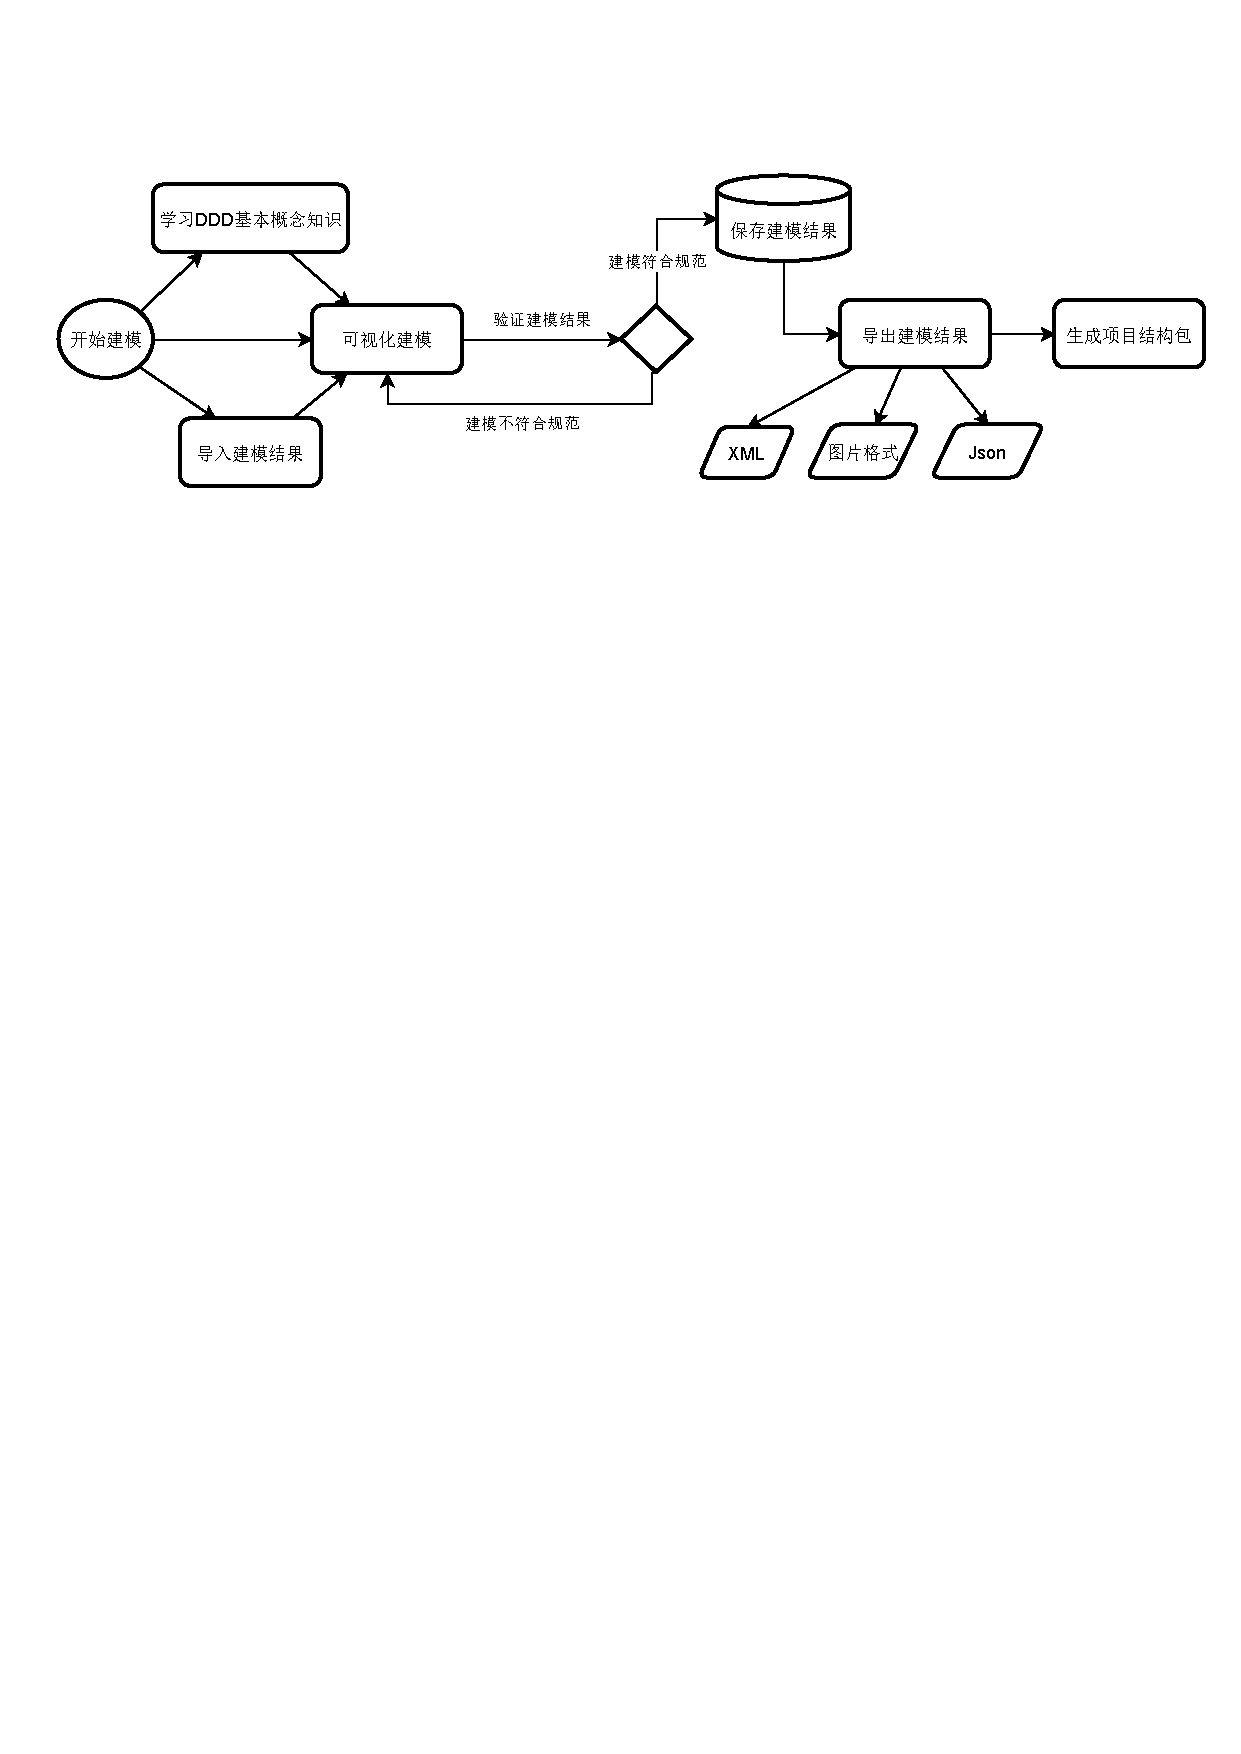
\includegraphics[width=0.8\textwidth]{FIGs/chapter3/toolprocess.pdf} %中括号中的参数是设置图片充满文档的大小,你也可以使用小数来缩小图片的尺寸。
%     \caption{框架支持工具业务流程} %caption是用来给图片加上图题的
%     \label{toolprocess} %这是添加标签,方便在文章中引用图片。
% \end{figure}%figure环境

\section{本章小结}

本章介绍了提出战术建模支持方法的研究过程及其结果。
其中研究过程包括文献综述、访谈和焦点小组,
文献综述部分对前期收集理论知识的目的和过程进行介绍,并为访谈和构建支持方法做准备工作;
访谈部分依据文献综述的成果,设计了问卷并对工业界内的领域驱动设计实践者进行访谈;
访谈后的初步产物作为焦点小组的输入,通过多次讨论,构建了战术建模支持方法。
研究结果包括由文献综述和访谈得到的战术建模指南,
即战术模式及属性、战术模式使用时机和实现技术;
还包括焦点小组讨论得出的战术建模语言。
上述战术建模指南和战术建模语言共同组成了本文提出的战术建模支持方法。




